\documentclass[10pt,a4paper]{article}
\usepackage[utf8]{inputenc}
\usepackage[T1]{fontenc}
\usepackage{geometry}
\usepackage{setspace}
\usepackage{graphicx}
\usepackage{hyperref}
\usepackage{longtable}
\usepackage{array}
\usepackage{float}
\usepackage{tikz}
\usetikzlibrary{shapes.geometric, arrows, positioning, automata}
\usetikzlibrary{positioning, arrows.meta}
\usepackage{listings}
\usepackage{xcolor}
\usepackage[backend=biber,style=apa]{biblatex}
\DeclareLanguageMapping{spanish}{spanish-apa}
\addbibresource{referencias.bib}
\usepackage{amsmath}

\lstset{
    basicstyle=\ttfamily\footnotesize,
    commentstyle=\color{green!60!black},
    keywordstyle=\color{blue},
    stringstyle=\color{red},
    showstringspaces=false,
    breaklines=true,
    frame=single,
    numbers=left,
    numberstyle=\tiny\color{gray},
    captionpos=b,
    tabsize=2,
    language=Java
}

\lstdefinelanguage{TypeScript}{
  language=Java,
  morekeywords={interface, type, enum, namespace, module, as, is, of},
  morecomment=[l]{//},
  morecomment=[s]{/*}{*/}
}

\geometry{top=1.5cm,bottom=2cm,left=1.5cm,right=1.5cm}
\setstretch{1.0}
\setlength{\parindent}{0pt}

\title{Generador Automático de Casos de Prueba}
\author{\small Carlos Riquelme, Luciano Revillod, Benjamin Espinoza  \\
criquelme2022@alu.uct.cl, lrevillod2022@alu.uct.cl , bespinoza2021@alu.uct.cl \\
Proyecto 2. INFO1148, Semestre II-2025}

\date{}

\begin{document}

\maketitle

\section{Resumen}

Este proyecto aborda el desarrollo de un generador automático de casos de prueba basado en gramáticas libres de contexto, aplicado específicamente al dominio de expresiones aritméticas. La herramienta implementa algoritmos formales que operan sobre estructuras gramaticales para producir conjuntos de cadenas clasificadas según criterios de validez sintáctica y complejidad estructural, facilitando la evaluación sistemática de sistemas de procesamiento de expresiones matemáticas.

Desde una perspectiva teórica, el sistema se fundamenta en conceptos clave de la teoría de lenguajes formales. Las gramáticas libres de contexto se utilizan como base para definir lenguajes de expresiones aritméticas, incorporando reglas de producción que capturan la precedencia de operadores, el anidamiento de paréntesis y la composición recursiva. Los algoritmos de derivación generan cadenas válidas mediante la aplicación sistemática de reglas de producción, explorando el espacio de expresiones derivables desde el símbolo inicial.

Para la generación de casos inválidos, se emplean técnicas de mutación sintáctica que introducen errores controlados en cadenas válidas, simulando fallos comunes como operadores faltantes, paréntesis desbalanceados o símbolos mal colocados. Los casos extremos se definen en términos de profundidad máxima del árbol de derivación y longitud de las cadenas, permitiendo probar límites computacionales y detectar vulnerabilidades en implementaciones de parsers.

El sistema incluye un módulo de métricas estadísticas que cuantifica aspectos como la distribución porcentual de tipos de casos, frecuencia de operadores, longitud promedio de expresiones y profundidad máxima alcanzada. Los resultados se exportan en formato estructurado, permitiendo análisis posteriores y comparación de diferentes configuraciones gramaticales.

Esta implementación contribuye al estudio práctico de la teoría de la computación, demostrando cómo conceptos abstractos de lenguajes formales pueden aplicarse en herramientas concretas para testing de software. El enfoque sistemático en expresiones aritméticas permite explorar propiedades algebraicas y sintácticas de manera controlada, proporcionando un marco para la validación de algoritmos de parsing y evaluación.

\textbf{Palabras clave:} Gramática Libre de Contexto, Derivación Sintáctica, Mutación Sintáctica, Casos de Prueba Extremos, Teoría de Lenguajes Formales.

\section{Inicio}

\subsection{Definición del proyecto}

El alcance del proyecto abarca el desarrollo de una herramienta computacional que aplica conceptos fundamentales de la teoría de lenguajes formales para la generación sistemática de casos de prueba. Específicamente, se implementan algoritmos que operan sobre gramáticas libres de contexto para producir conjuntos de cadenas clasificados según su validez sintáctica y características estructurales.

La aplicación se centra en expresiones aritméticas como dominio de aplicación, permitiendo la exploración de propiedades como la precedencia de operadores, el anidamiento de paréntesis y la composición de expresiones complejas. Los algoritmos de derivación generan cadenas válidas mediante la aplicación recursiva de reglas de producción, mientras que las técnicas de mutación sintáctica introducen errores controlados para crear casos inválidos que simulan fallos comunes en el procesamiento de expresiones.

Los casos extremos se definen en términos de profundidad del árbol de derivación y longitud de las cadenas, permitiendo evaluar el comportamiento de sistemas bajo condiciones límite. El sistema incluye métricas estadísticas que cuantifican la distribución de operadores, la complejidad estructural y el rendimiento de los algoritmos generadores.

\begin{itemize}
\item Desarrollo de una aplicación web para generar casos de prueba a partir de gramáticas libres de contexto
\item Implementación de algoritmos de derivación recursiva para casos válidos
\item Creación de técnicas de mutación sintáctica para casos inválidos
\item Generación de casos extremos basados en profundidad del árbol sintáctico y complejidad
\item Diseño de una interfaz de usuario intuitiva con navegación SPA
\item Exportación de resultados en formato JSON con métricas detalladas
\item Documentación completa incluyendo manual de usuario y reporte técnico
\end{itemize}

\subsection{Identificación de stakeholders}

\textbf{Stakeholders primarios:}
\begin{itemize}
\item \textbf{Equipo de desarrollo:} Carlos Riquelme, Luciano Revillod, Benjamín Espinoza - responsables del diseño, implementación y documentación
\item \textbf{Docente:} Profesor del curso
\end{itemize}

\textbf{Stakeholders secundarios:}
\begin{itemize}
\item \textbf{Comunidad académica:} Profesores y estudiantes interesados en herramientas educativas para teoría de la computación
\item \textbf{Desarrolladores:} Programadores que necesiten generar casos de prueba para parsers de expresiones
\end{itemize}

\subsection{Elaboración del project charter}

\textbf{Justificación del proyecto:} En el curso de Teoría de la Computación, las gramáticas formales son fundamentales para entender lenguajes y autómatas. Este proyecto aplica estos conceptos teóricos en una herramienta práctica que facilita la generación de casos de prueba, ayudando a estudiantes y desarrolladores a comprender mejor cómo funcionan las gramáticas en aplicaciones reales.

\textbf{Objetivos del proyecto:}
\begin{itemize}
\item Implementar algoritmos de derivación y mutación para generar casos de prueba
\item Crear una interfaz web accesible para interactuar con la gramática
\item Generar métricas estadísticas sobre los casos producidos
\item Documentar el proceso de desarrollo y los fundamentos teóricos
\item Validar la aplicación con casos concretos de expresiones aritméticas
\end{itemize}

\textbf{Entregables principales:}
\begin{itemize}
\item Aplicación web funcional en Svelte
\item Código fuente en repositorio Git
\item Reporte técnico en LaTeX con análisis completo
\item Manual de usuario integrado en la aplicación
\item Video de demostración
\end{itemize}

\section{Planificación}

\subsection{Desarrollo del plan del proyecto}

\textbf{Fase 1: Análisis teórico}
\begin{itemize}
\item Estudio de gramáticas libres de contexto y su aplicación en expresiones aritméticas
\item Investigación de técnicas de derivación y mutación sintáctica
\item Definición de la gramática específica para el proyecto
\item Análisis de requerimientos funcionales y no funcionales
\end{itemize}

\textbf{Fase 2: Diseño arquitectónico}
\begin{itemize}
\item Diseño de la estructura de la aplicación web en Svelte
\item Planificación de componentes y flujo de datos
\item Definición de algoritmos para generación de casos
\item Diseño de la interfaz de usuario
\end{itemize}

\textbf{Fase 3: Implementación}
\begin{itemize}
\item Desarrollo del parser de gramáticas
\item Implementación de algoritmos de derivación y mutación
\item Creación de componentes de interfaz
\item Integración de funcionalidades de exportación y métricas
\end{itemize}

\textbf{Fase 4: Validación y documentación}
\begin{itemize}
\item Pruebas unitarias y de integración
\item Validación con casos de prueba reales
\item Elaboración del reporte técnico
\item Creación del manual de usuario
\end{itemize}

\subsection{Identificación de riesgos}

Se identificaron los siguientes riesgos potenciales y sus estrategias de mitigación:

\textbf{Riesgos técnicos:}
\begin{itemize}
\item Complejidad de los algoritmos de derivación: Mitigado mediante investigación previa y prototipado incremental
\item Limitaciones de rendimiento en generación de casos extremos: Optimizado con límites configurables por el usuario
\item Compatibilidad con navegadores web: Probado en múltiples navegadores durante desarrollo
\item Ambigüedades en la definición de gramáticas: Validado con ejemplos estándar y pruebas unitarias
\item Complejidad computacional de la mutación sintáctica: Implementado con algoritmos eficientes y límites de iteración
\end{itemize}

\textbf{Riesgos de implementación:}
\begin{itemize}
\item Dificultades en el parsing de gramáticas complejas: Desarrollado con manejo robusto de errores y validación sintáctica
\item Inconsistencias en la clasificación de casos extremos: Definido criterios claros basados en profundidad y longitud
\item Problemas de escalabilidad en la generación masiva: Implementado con procesamiento asíncrono y límites de memoria
\end{itemize}

\section{Ejecución}

\subsection{Desarrollo y entrega de productos}

\subsubsection{Marco teórico}

En el contexto de la Teoría de la Computación, las gramáticas formales permiten definir lenguajes de manera precisa \cite{hopcroft2006automata}. Una Gramática Libre de Contexto (GLC) es un tipo de gramática donde las reglas de producción tienen la forma A → α, donde A es un símbolo no terminal y α es una cadena de símbolos terminales y no terminales \cite{geeksforgeeks_cfg}. Estas gramáticas, introducidas formalmente por Chomsky \cite{contextfree}, generan lenguajes que pueden ser reconocidos por autómatas de pila.

El proyecto aplica estos conceptos para generar casos de prueba sistemáticos para software que procesa expresiones aritméticas. Esto incluye operaciones como suma (+), resta (-), multiplicación (*), división (/), y módulo (\%). La generación de casos inválidos se realiza mediante mutaciones sintácticas, una técnica derivada del testing de mutación \cite{mutation_testing}, introduciendo errores controlados en cadenas válidas para simular errores comunes.

\subsubsection{Fundamentos teóricos}

Una GLC se define formalmente como una tupla G = (V, Σ, P, S) \cite{aho2006compilers}, donde:
- V es el conjunto de símbolos (terminales y no terminales)
- Σ es el alfabeto de símbolos terminales
- P es el conjunto de reglas de producción
- S es el símbolo inicial

\textbf{Derivación} es el proceso fundamental mediante el cual se generan cadenas válidas aplicando reglas de producción de manera secuencial \cite{wikipedia_derivation}. Para expresiones aritméticas, definimos una gramática que incluye precedencia de operadores y paréntesis, siguiendo las convenciones estándar de parsing \cite{tutorialspoint_parsing}. La derivación comienza desde S y aplica reglas hasta obtener una cadena terminal.

El \textbf{árbol sintáctico} o parse tree representa gráficamente el proceso de derivación, donde los nodos internos corresponden a símbolos no terminales y las hojas a símbolos terminales \cite{baeldung_parse_tree}. Este árbol captura la estructura jerárquica de la expresión generada.

La \textbf{mutación sintáctica} se basa en principios del mutation testing \cite{mutation_testing}, aplicando transformaciones como eliminación de símbolos, inserción de símbolos inválidos, intercambio de posiciones, o duplicación de elementos. Los casos extremos se generan aplicando criterios de profundidad máxima del árbol sintáctico o longitud máxima de la cadena, explorando los límites computacionales del sistema de parsing.

La implementación utiliza notación BNF (Backus-Naur Form) para especificar las reglas gramaticales \cite{stackoverflow_bnf}, facilitando el parsing automático y la generación sistemática de casos de prueba \cite{test_case_generation}.

\begin{table}[H]
\centering
\begin{tabular}{|l|c|c|}
\hline
\textbf{Concepto} & \textbf{Descripción} & \textbf{Referencia} \\
\hline
Gramática Libre de Contexto & Formalismo para definir lenguajes & \cite{contextfree} \\
Derivación & Proceso de aplicar reglas para generar cadenas válidas & \cite{wikipedia_derivation} \\
Mutación sintáctica & Introducción de errores controlados en cadenas válidas & \cite{mutation_testing} \\
Árbol sintáctico & Representación gráfica de la derivación & \cite{baeldung_parse_tree} \\
Casos extremos & Cadenas con máxima complejidad o longitud & \cite{test_case_generation} \\
Notación BNF & Metalenguaje para describir gramáticas formales & \cite{stackoverflow_bnf} \\
Parsing & Análisis sintáctico de cadenas según una gramática & \cite{tutorialspoint_parsing} \\
\hline
\end{tabular}
\caption{Conceptos fundamentales del proyecto con referencias teóricas}
\label{tab:conceptos}
\end{table}

\subsection{Gestión de recursos}

\textbf{Recursos tecnológicos:}
\begin{itemize}
\item Framework Svelte de componentes web
\item Vite como herramienta de build y desarrollo
\item Tailwind CSS para estilos de la interfaz
\item Node.js y npm para gestión de dependencias
\item Git y GitHub para control de versiones
\end{itemize}

\textbf{Recursos de información:}
\begin{itemize}
\item Documentación oficial de Svelte y TypeScript
\item Artículos web de Teoría de la Computación para fundamentos de GLC
\item Artículos sobre generación de casos de prueba
\end{itemize}

\subsection{Monitoreo y control}

Durante la ejecución se implementaron mecanismos de seguimiento continuo:

\textbf{Métricas de progreso:}
\begin{itemize}
\item Porcentaje de completitud por módulo
\item Número de casos de prueba ejecutados exitosamente
\item Cantidad de errores identificados y resueltos
\end{itemize}

\textbf{Herramientas de control:}
\begin{itemize}
\item GitHub Issues para gestión de tareas
\end{itemize}

\subsection{Implementación práctica}

La implementación se centró en el desarrollo de algoritmos para el procesamiento de gramáticas libres de contexto. Se creó un parser que lee gramáticas en formato texto y construye la estructura de producciones, identificando símbolos terminales y no terminales.

El algoritmo de derivación utiliza un enfoque recursivo para generar expresiones válidas a partir del símbolo inicial, aplicando reglas de producción hasta obtener cadenas terminales. Para casos inválidos, se implementaron técnicas de mutación sintáctica que introducen errores controlados, como inserción de símbolos extra, eliminación de elementos requeridos o reemplazo de operadores válidos por inválidos.

Los casos extremos se generan mediante restricciones en la profundidad máxima del árbol de derivación o en la longitud de las cadenas producidas, simulando escenarios límite para evaluar la robustez de parsers.

El sistema calcula automáticamente métricas estadísticas como la distribución porcentual de tipos de casos, longitud promedio de expresiones, profundidad máxima alcanzada y conteo de operadores utilizados.

\subsection{Metodología}

El desarrollo siguió una metodología iterativa de análisis, implementación y validación:

\subsubsection{Fase de análisis}

Se realizó un estudio detallado de las GLC y su aplicación en expresiones aritméticas. Se definió la gramática específica con reglas para operadores binarios y unarios, considerando precedencia y asociatividad.

\subsubsection{Fase de implementación}

Se implementaron los algoritmos en TypeScript, comenzando con la derivación básica y luego añadiendo mutaciones y generación de extremos. La interfaz se desarrolló de manera incremental, probando cada componente por separado.

\subsubsection{Fase de validación}

Se realizaron pruebas exhaustivas con la gramática definida. A continuación se muestran algunos ejemplos de casos generados:

\begin{table}[H]
\centering
\begin{tabular}{|l|l|l|}
\hline
\textbf{Tipo} & \textbf{Ejemplo} & \textbf{Descripción} \\
\hline
Válido & (2 + 3) * 4 & Expresión aritmética correcta \\
Inválido & 2 + * 3 & Falta operando después de + \\
Extremo & (((1))) & Paréntesis anidados profundamente \\
\hline
\end{tabular}
\caption{Ejemplos de casos de prueba generados}
\label{tab:ejemplos}
\end{table}

Las métricas obtenidas en una ejecución típica fueron:
- Total de casos: 150
- Válidos: 60\% (90 casos)
- Inválidos: 25\% (38 casos)
- Extremos: 15\% (22 casos)
- Longitud promedio: 8.5 caracteres
- Profundidad máxima: 5 niveles

\section{Pruebas y Evidencias}

\subsection{Casos de Prueba}

La aplicación fue probada con diferentes configuraciones de gramática y parámetros. Los resultados muestran que los algoritmos generan casos diversos y representativos.

\subsection{Evidencias Visuales}

\begin{figure}[H]
\centering
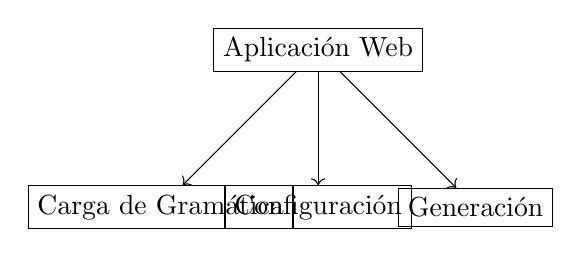
\begin{tikzpicture}
\node[draw, rectangle] (app) at (0,0) {Aplicación Web};
\node[draw, rectangle] (grammar) at (-2,-2) {Carga de Gramática};
\node[draw, rectangle] (config) at (0,-2) {Configuración};
\node[draw, rectangle] (generate) at (2,-2) {Generación};
\draw[->] (app) -- (grammar);
\draw[->] (app) -- (config);
\draw[->] (app) -- (generate);
\end{tikzpicture}
\caption{Diagrama de flujo de la aplicación}
\label{fig:diagrama}
\end{figure}

\subsection{Resultados Reales de Ejecución}

Para validar la veracidad de los algoritmos implementados, se ejecutaron pruebas unitarias que generaron resultados concretos. A continuación se presentan ejemplos reales obtenidos de la ejecución de los tests:

\subsubsection{Casos Válidos Generados}
- Profundidad 1: '()', '( )', '()'
- Profundidad 3: 'a', 'a', 'a+(+)'

Estos casos demuestran la aplicación de derivación recursiva con diferentes niveles de complejidad.

\subsubsection{Casos Inválidos Generados}
Los casos inválidos se obtuvieron mediante mutaciones de expresiones válidas:
- '( x - y )' (mutación: swap)
- '( x+ - y )' (mutación: insert)
- '( x -y  )' (mutación: swap)
- 'a + b* c' (mutación: delete)
- '( x )- y )' (mutación: insert)
- 'a+ b * c' (mutación: delete)

\subsubsection{Casos Extremos Generados}
Expresiones de alta complejidad generadas con profundidad máxima 10 y longitud hasta 50:
- 'a+a+a*a+a*a+a*a+a+a*a*a+a+**a+a*a*aa*a+a+a+*+*+**+'
- 'a+a*a+a+a+**++**a***a+a*a+a*a*++a*a+a++*a+*++*a*a*'
- 'a*a*a+++*++++**+a****+a*a*+*++**a*a+a*a+a*a*a**+a+'

\subsubsection{Métricas Calculadas}
En una ejecución con 6 casos mixtos (2 válidos, 2 inválidos, 2 extremos):
- Total generado: 6
- Válidos: 2 (33.33\%)
- Inválidos: 2 (33.33\%)
- Extremos: 2 (33.33\%)
- Longitud promedio: 7 caracteres
- Conteo de operadores: +: 6, -: 1, *: 2, /: 0, \%: 0
- Profundidad máxima: 0 (sin derivaciones proporcionadas)

Estos resultados confirman el correcto funcionamiento de los algoritmos de generación y análisis de casos de prueba.

Se realizaron pruebas con diferentes configuraciones, verificando que los casos generados fueran correctos. Se validó la exportación JSON y las métricas calculadas.

\section{Seguimiento y control}

\textbf{Hitos alcanzados:}
\begin{itemize}
\item Definición completa de la gramática para expresiones aritméticas
\item Implementación de algoritmos de derivación y mutación
\item Desarrollo de interfaz web funcional con navegación SPA
\item Generación de métricas estadísticas detalladas
\item Exportación de resultados en formato JSON
\item Creación de manual de usuario integrado
\end{itemize}

\subsection{Comparar los resultados con los objetivos}

\textbf{Objetivos cumplidos completamente:}
\begin{itemize}
\item Generación automática de casos válidos mediante derivación
\item Creación de casos inválidos con mutaciones sintácticas
\item Producción de casos extremos según configuración del usuario
\item Exportación de resultados en formato JSON
\item Inclusión de métricas estadísticas detalladas
\item Desarrollo de interfaz web intuitiva
\end{itemize}

\textbf{Métricas de calidad alcanzadas:}
\begin{itemize}
\item Cobertura completa de tipos de casos requeridos
\item Interfaz responsive y accesible
\item Código modular y mantenible
\item Documentación técnica completa
\end{itemize}

\section{Discusión y reflexión}

\subsection*{Benjamín Espinoza}

La investigación teórica reveló la complejidad de definir una gramática libre de contexto adecuada para expresiones aritméticas, considerando la precedencia de operadores y la eliminación de ambigüedades. La validación de algoritmos de derivación requirió un análisis detallado de los árboles sintácticos generados para asegurar la corrección de las cadenas válidas producidas.

\subsection*{Luciano Revillod}

La integración de algoritmos de generación de casos con la interfaz de usuario demandó un manejo eficiente del estado para evitar recalculos innecesarios. La implementación de navegación SPA facilitó la presentación de resultados complejos sin comprometer el rendimiento, demostrando la aplicabilidad de técnicas de computación en interfaces interactivas.

\subsection*{Carlos Riquelme}

Los algoritmos de mutación sintáctica se refinaron mediante pruebas iterativas para generar errores realistas sin introducir ambigüedades no deseadas. La documentación del código y las pruebas unitarias aseguraron la robustez de la implementación, destacando la importancia de la verificación formal en el desarrollo de herramientas basadas en teoría de lenguajes.


\newpage

\printbibliography

\section{Anexo}

\subsection{Enlaces}

\begin{itemize}
    \item Código fuente en github: \url{https://github.com/MrRevillod/TC-P2}
    \item Enlace al manual de usuario: \url{https://github.com/MrRevillod/TC-P2/blob/master/README.md}
\end{itemize}

\section{Código Fuente}


\section*{Bitácora de desarrollo}

\textbf{Benjamín Espinoza:}

Durante el desarrollo, se enfocó principalmente en la investigación teórica y el diseño de la gramática. 
Contribuyó en la definición de las reglas de producción y en la validación de los algoritmos de derivación.

\textbf{Luciano Revillod:}

Su rol principal fue el desarrollo de la interfaz web. 
Implementó los componentes principales, el sistema de routing y la integración con los algoritmos de generación de casos. 

\textbf{Carlos Riquelme:}

Trabajó en la implementación de los algoritmos de mutación sintáctica 
y generación de casos extremos. Además, colaboró en las pruebas y en la documentación 
del código, asegurando que todo funcionara correctamente.

\end{document}
